\section{Applying Comparative Concepts}

In the previous section we have compared cases from two languages as if they were from a commensurable descriptive category.
In this section, we take the other view that Universal Dependencies defines comparative concepts and that the various treebanks are annotated with these concepts.
%However, we will now try to prototype, that is, find a typical vector representation of each case, so as to check if the cases syntactically match their supposed theoretical definition represented in table \ref{table:desc_case}

\begin{table}
\centering
\begin{NiceTabular}{p{.24\columnwidth}p{.44\columnwidth}p{.15\columnwidth}}
    \toprule
    Case & Description & DepRel\\
    \midrule
    \textsc{Nominative} & Subject of a clause. & \tt nsubj \\
    \midrule
    \textsc{Accusative} & Direct object of transitive verbs. & \tt obj \\
    \midrule
    \textsc{Absolutive} & Subject of intransitive verbs and object of transitive verbs. & \tt nsubj \newline obj \\
    \midrule
    \textsc{Ergative} & Subject of transitive verbs. & \tt nsubj \\
    \midrule
    \textsc{Genitive} & Noun complement, typically possessor. & \tt nmod \\
    \midrule
    \textsc{Dative} & Indirect object of verbs, typically recipient of giving verbs. & \tt iobj \\
    \bottomrule
\end{NiceTabular}
    \caption{Ideal description of a few cases and corresponding UD's dependency relations.}
    \label{table:desc_case}
\end{table}

To do so, we consider that each comparative case is associated with a random variable taking values from the probability distributions over the set of dependency relations to a word's governor. 
We know each of these random variables through a number of realisations (the vector representations of the considered case across all corpora where it is present). 
That is, this random variable maps a language to a probability distribution over the dependency relations reaching words marked with that case. 

Then, to compute the profile of the comparative cases, we compute the expectancy of the random variables associated to each case. 
Since the values of the random variables are distributions we also compute the barycentre of the realisations of a variable for the Wasserstein $1$-distance (or Earth Mover's Distance). 
We will denote the latter by \emph{Wasserstein barycentre}.
%We obtain the distribution represented in table \ref{table:prototypes} when considering only nouns.

\begin{table*}[h!]
\centering
\renewcommand{\arraystretch}{1.3}
\begin{NiceTabular}{llccccc}
        \bf Case & \bf Average &\tt iobj & \tt nmod & \tt nsubj & \tt obj & \tt obl\\
        \multirow[c]{2}{*}{\bf\sc Abs}  & Uniform    & 0.1 & 3.3 & 27.2 & 36.7 & 22.4\\
                                        & Wasserstein & 0.0 & 1.6 & 28.6 & 52.2 & 11.2\\

        \multirow[c]{2}{*}{\bf\sc Erg}  & Uniform    & 0.0 & 0.7 & 92.4 & 0.5 & 5.9\\
                                        & Wasserstein & 0.0 & 0.5 & 97.6 & 1.4 & 0.3\\

        \multirow[c]{2}{*}{\bf\sc Nom}  & Uniform    & 0.1 & 8.0 & 55.6 & 7.4 & 5.0\\
                                        & Wasserstein & 0.0 & 4.9 & 65.4 & 9.3 & 3.8\\

        \multirow[c]{2}{*}{\bf\sc Acc}  & Uniform    & 0.6 & 7.8 & 3.8 & 62.5 & 20.5\\
                                        & Wasserstein & 0.0 & 7.2 & 1.9 & 57.6 & 25.9\\

        \multirow[c]{2}{*}{\bf\sc Gen}  & Uniform    & 0.9 & 67.4 & 3.9 & 5.6 & 14.9\\
                                        & Wasserstein & 0.0 & 72.9 & 3.1 & 4.5 & 17.9\\

        \multirow[c]{2}{*}{\bf\sc Dat}  & Uniform    & 14.4 & 14.9 & 1.9 & 0.0 & 57.2\\
                                        & Wasserstein & 19.0 & 16.4 & 0.5 & 0.0 & 60.5\\

        \multirow[c]{2}{*}{\bf\sc Loc}  & Uniform    & 0.0 & 16.6 & 0.9 & 1.7 & 69.6\\
                                        & Wasserstein & 0.0 & 18.8 & 0.0 & 0.0 & 76.2\\

        \multirow[c]{2}{*}{\bf\sc Ins}  & Uniform    & 0.0 & 17.2 & 1.4 & 0.0 & 66.0\\
                                        & Wasserstein & 0.0 & 21.3 & 0.0 & 0.0 & 73.8\\

        \multirow[c]{2}{*}{\bf\sc Abl}  & Uniform    & 0.0 & 16.5 & 1.3 & 1.0 & 70.0\\
                                        & Wasserstein & 0.0 & 17.2 & 0.0 & 0.0 & 78.5\\
        \CodeAfter
        \begin{tikzpicture}
                \foreach \i in {2, 4,...,19} {\draw[black] (1|-\i) -- (8|-\i);}
                \draw[black] (2|-1) -- (2|-20);
                \foreach \i in {3, 5,..., 19} {\draw[gray, dashed] (2|-\i) -- (8|-\i);}
        \end{tikzpicture}
\end{NiceTabular}
\caption{Distributions of the most representative dependency relations for a few cases as computed on nouns. 
Uniform corresponds to the average profile assuming uniform weighting of each corpus profile.
Wasserstein corresponds to barycentres computed with the Wasserstein metric taking into consideration that case profiles are not any vector, but actual probability distributions.}
\label{table:prototypes}
\end{table*}

Table \ref{table:prototypes} gives the representations of the expected distributions of a few selected comparative cases.
%Here we most importantly see that the expected representation is very similar to the real one. 
The representations are mostly aligned with our expectations.
But we can still notice a few interesting facts.
The \textsc{ergative} is much more strongly associated with being a subject than the \textsc{nominative} is.
There may be a few different reasons to that.
First, some language like Turkish use the nominative/accusative distinction also to mark a definite/indefinite distinction on the object, with the accusative being kept for definite objects.
Another possibility is that when a language has case marking but does not make distinction between subjects and objects such as Irish, it is by default assumed to be nominative-accusative, with the nominative assuming both syntactic roles\footnote{In the eventuality that it would be considered an ergative-absolutive language, the default case would likely be called absolutive rather than ergative anyway.}.

Another interesting fact is that the \textsc{dative}'s main role is not that of indirect object but rather of oblique. 
This comes from the strong limitations that UD imposes on the use of the \texttt{iobj} relation.
But still, \textsc{dative} is virtually the only case to assume that role.

However, while this representation allows us to distinguish many cases syntactically, it doesn't allow to distinguish all cases. 
More specifically, some cases work in the same syntactic constructions and thus are mostly distinguished through their semantic properties. 
For example, the Finnish \scsf{ellative} and \scsf{illative} are used to signify that a movement respectively comes from a place or into a place. In the sentence \textsl{I went into his house}, \textsl{house} would be in illative in finnish, while in \textsl{I come back from his house}, \textsl{house} would be in ellative. 

This is exactly what we see for non-core cases.
\textsc{Locative}, \textsc{instrumental} and \textsc{ablative} have very similar profiles, essentially distributed between oblique complements of verbs and nominal modifiers or nouns.



%This comes first from the theoretical definition of cases: indeed, if a case is well defined in a language, the case semantically (and often syntactically) equivalent in another language has chances to be named the same. 

To check the representativeness of a comparative case $P$ of its realisations across treebanks, we compute its energy $E$:
\begin{align}
    P = \arg\min_{x} E\left(x, \left(x_{i}\right)_{i \in \left\llbracket 1, n\right\rrbracket}\right) \\ 
    E\left(x, \left(x_{i}\right)_{i \in \left\llbracket 1, n\right\rrbracket}\right) = \frac{1}{n}\sum_{i = 1}^{n} d(x, x_{i})
\end{align}
The energies associated to the two barycenters are of the same magnitude, with the wasserstein barycenter being more exacerbated as can be seen in figure \ref{fig:prototypes} for the \textsc{accusative} case.

The x-axis represents the different dependency relations leading to nouns in the accusative, the exact list is given in the appendix for convenience. 
It represents in red the uniform mean of distributions (the expectancy of the variable), in yellow the barycenter of the distributions associated to the Wasserstein $1$-distance and in purple the (unnormalized for graphical purposes) apparition frequency. 

We can notably see that for uniform mean some relations are represented because very present in a few languages while this is not the case for the Wasserstein barycenter, which is more centered on the deprels present in a lot of languages. % !!!! tell at which index so that people can see it too

\begin{figure}[h!]
    \centering
    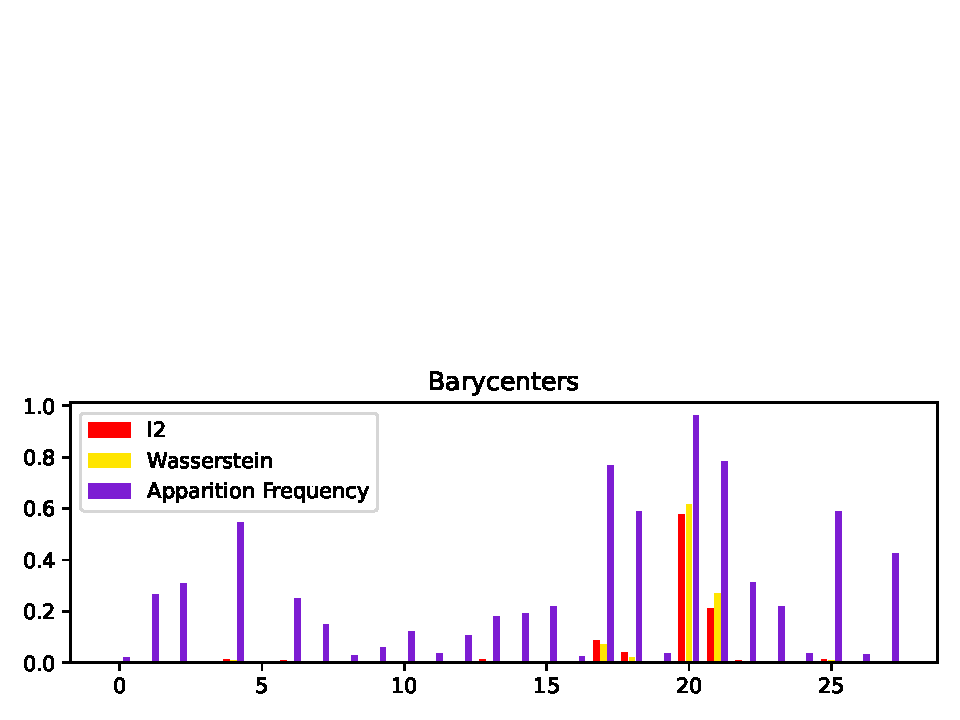
\includegraphics[width=\linewidth]{Images/Base_Nouns_Wasserstein_Barycenter_Acc.pdf}
    \caption{Representation of the uniform barycentre in red and the Wasserstein barycentre in yellow for the comparative \textsc{accusative} case.
    In purple is represented the proportion of treebanks that associate a given dependency relation with nouns in the accusative from the set of treebanks that inflect their nouns for case.}
    \label{fig:prototypes}
    % we need to know what the x means
\end{figure}

%Thus we show that there is a general structure for cases with the same name across languages, and that some of those can be quantitatively distinguished, but this method is not able to get visible distinctions. 

% en fait non, on a pas fait ça ^^, on a pas mis les distance entres les cas prototypique et les cas de chaque langue, ou potentiellement certains sont pas alignés avec leur nom....

% mais on le fait un peu avec le knn de la section suivante